\section{Evaluation} \label{sec:evaluation}
\todo[inline, color=red]{Britta}

\subsection{Tasks} \label{sec:tasks}
\todo[inline, color=yellow]{Anna}
In the supermarket are four different tasks the user has to do. In every tasks a object has to be selected and placed on a target area. If the correct object is placed, the target area will change the color to signal that the tasks is successful done. In the script \textit{TargetTest.cs}, which will be a component of the target object, will be recognized when the target object hits the target area. At this moment the texture of target area will be changed and the measurement will be stopped. More information about the measurement will be mentioned in section \ref{sec:measurement}.\\
In the first three tasks the user has to select different objects. In this tasks the user decides which methods he/she uses. The selected methods should differ depending on the tasks. In these tasks objects far away as well as closely should be picked. \\
The tasks will be shown on the controller similar to the selfteaching which the user is already aware of, shown in the following figure. 

\begin{figure}[H] 
	\center 
	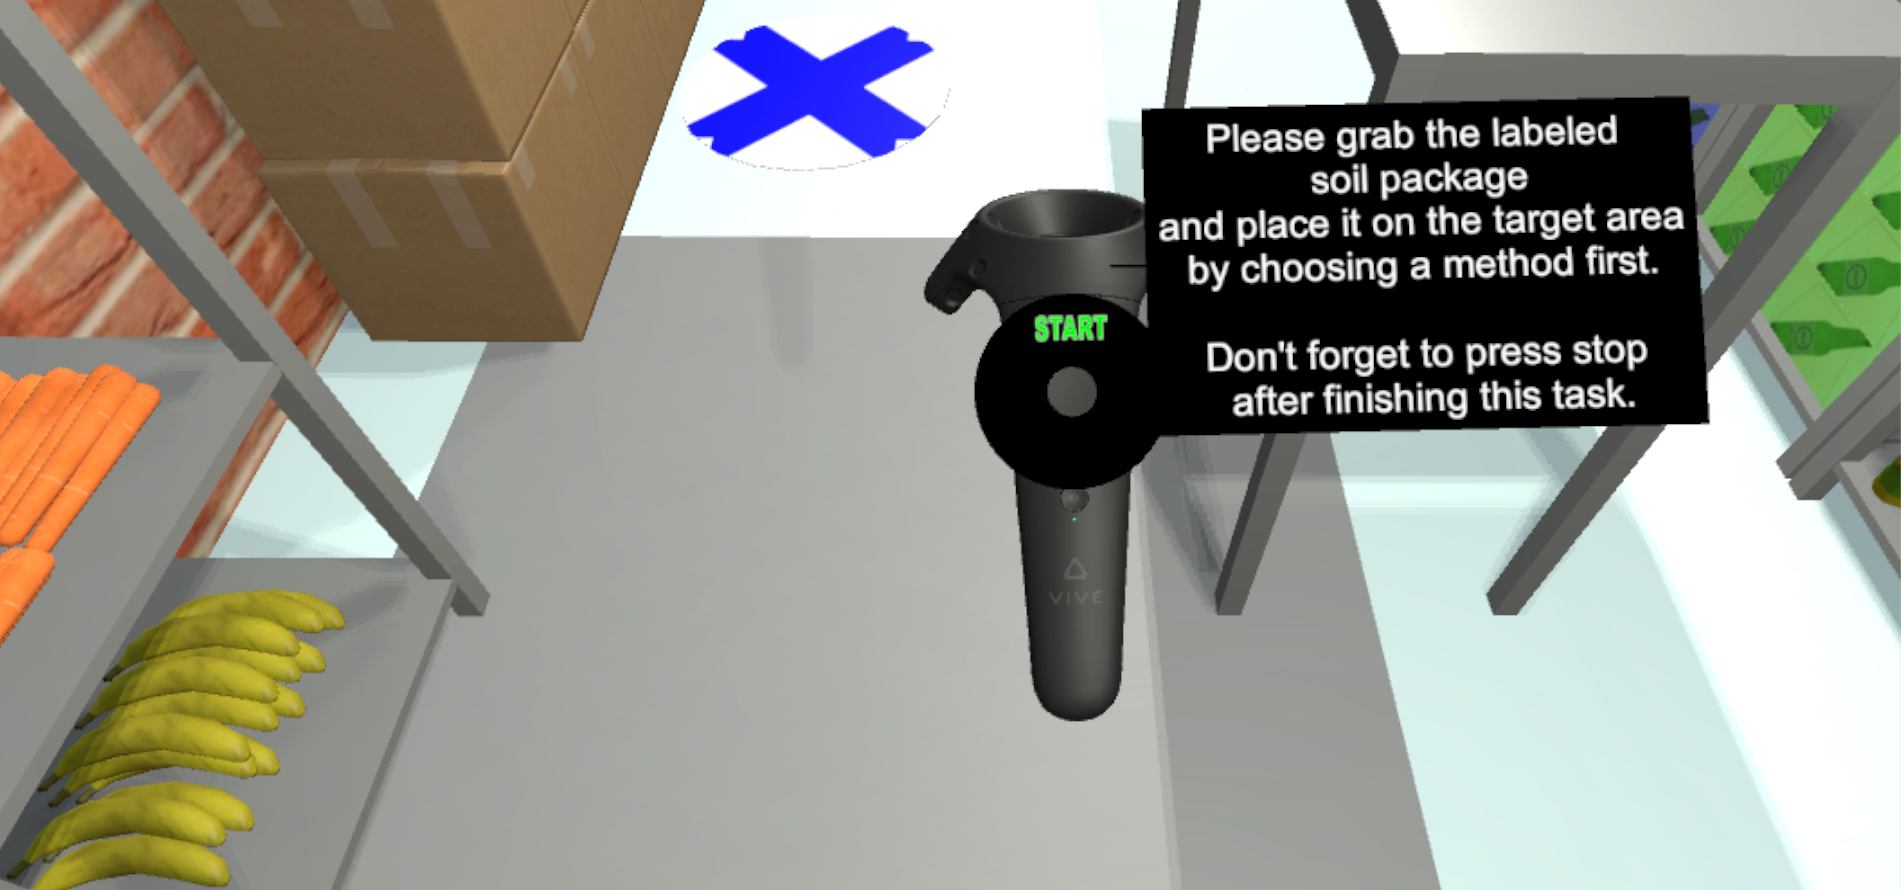
\includegraphics[width=12cm]{Images/TaskContreoller.PNG}
	\caption[Task shown on the controller]{Task shown on the controller}
	\label{fig:taskC}
\end{figure} 

The text for the tasks are saved in a CSV-file, similar to the selfteaching, see section \ref{sec:selfteaching}. The implementation is also related to the selfteaching and implemented in the script \textit{showTasks.cs}.

\begin{figure}[H] 
	\center 
	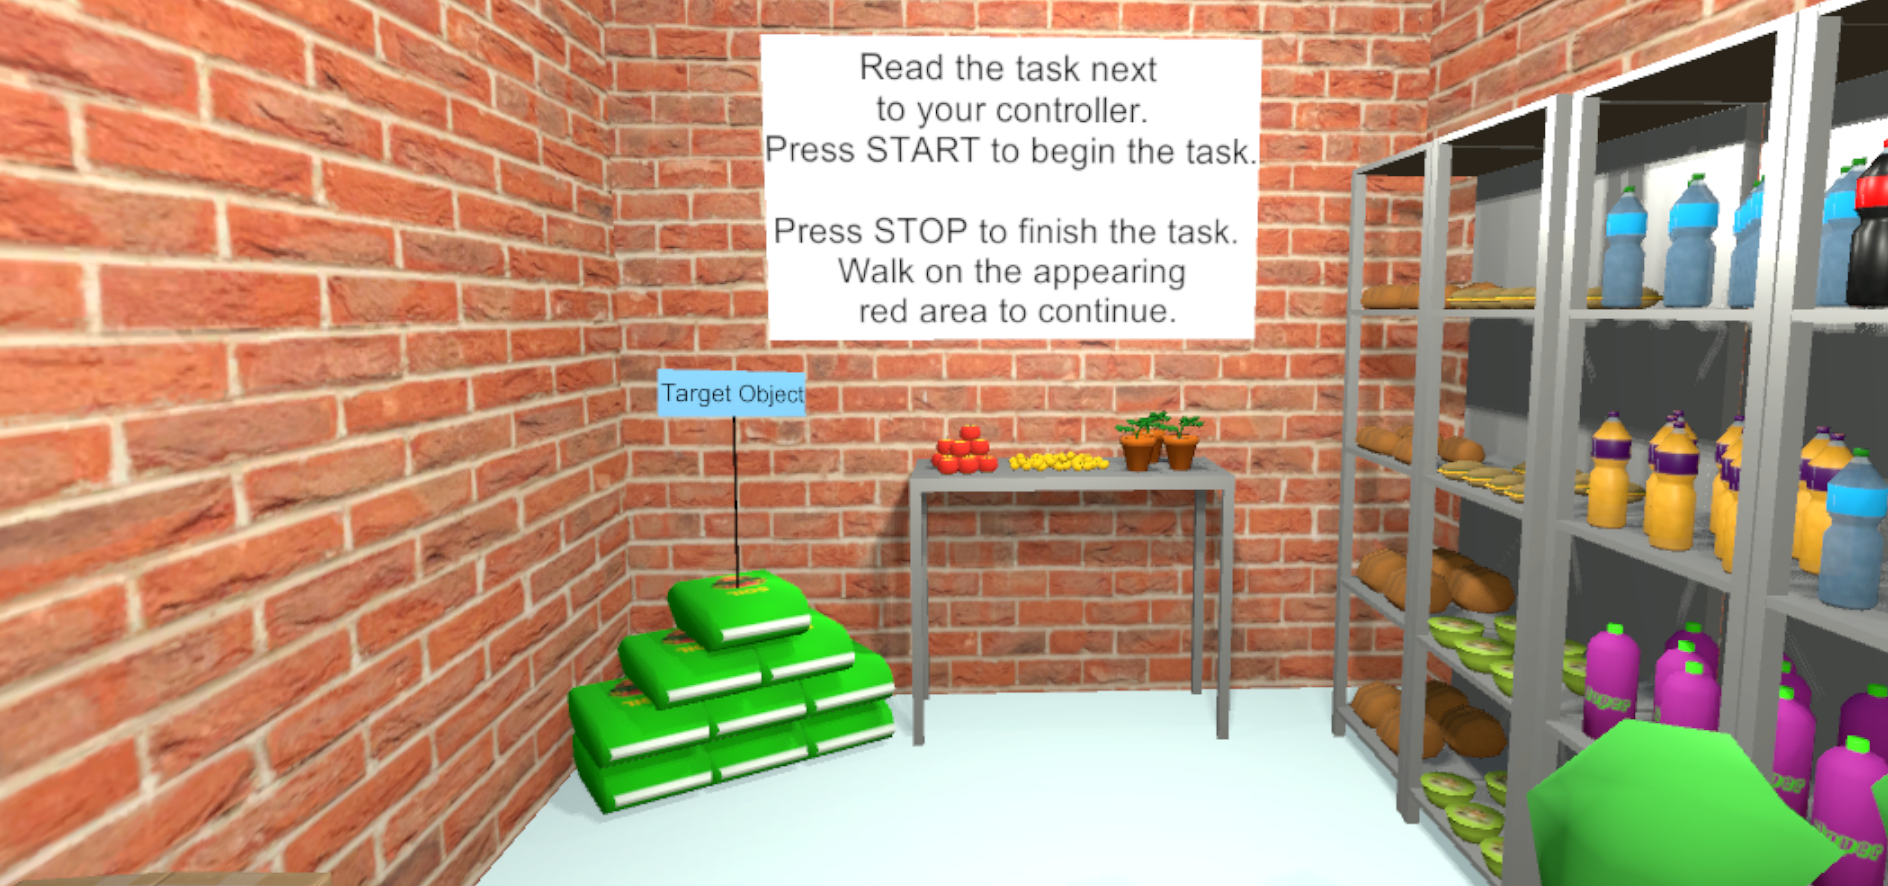
\includegraphics[width=12cm]{Images/TaskWall_1.PNG}
	\caption[Additional informations on the wall]{Additional informations on the wall}
	\label{fig:taskW1}
\end{figure}

To give the user some more information a information board within the supermarket is established, see figure \ref{fig:taskW1}. In the first tasks there are only shown some basic informations.\\
The last tasks will be repeated with every available method. That means, that the user has to pick up the same object five times. This object is so placed that the user could use close as well as far range methods. The methods are fix implemented, in order like in table \ref{tab: OrderMethods}. The methods will already  be activated as soon as the user presses start. \\

\begin{table}[h]
\centering
 \begin{tabular}{|c|c|}
  Number of subtask & Method  \\ \hline
  1 & Close Range: Touch Grab  \\
  2 & Close Range: Wand Grab  \\
  3 & Far Range: Extendable Ray  \\
  4 & Close Range: Proximity Grab  \\
  5 & Far Range: Raycast \\
   \end{tabular}
  \caption[Order of methods in the last task]{Order of methods in the last task}
	\label{tab: OrderMethods}
 \end{table}

To help the user to figure out what method will be activated the name of the method will be shown on the information board as soon as  he/she is in the new scene, like in the following figure. 

\begin{figure}[H] 
	\center 
	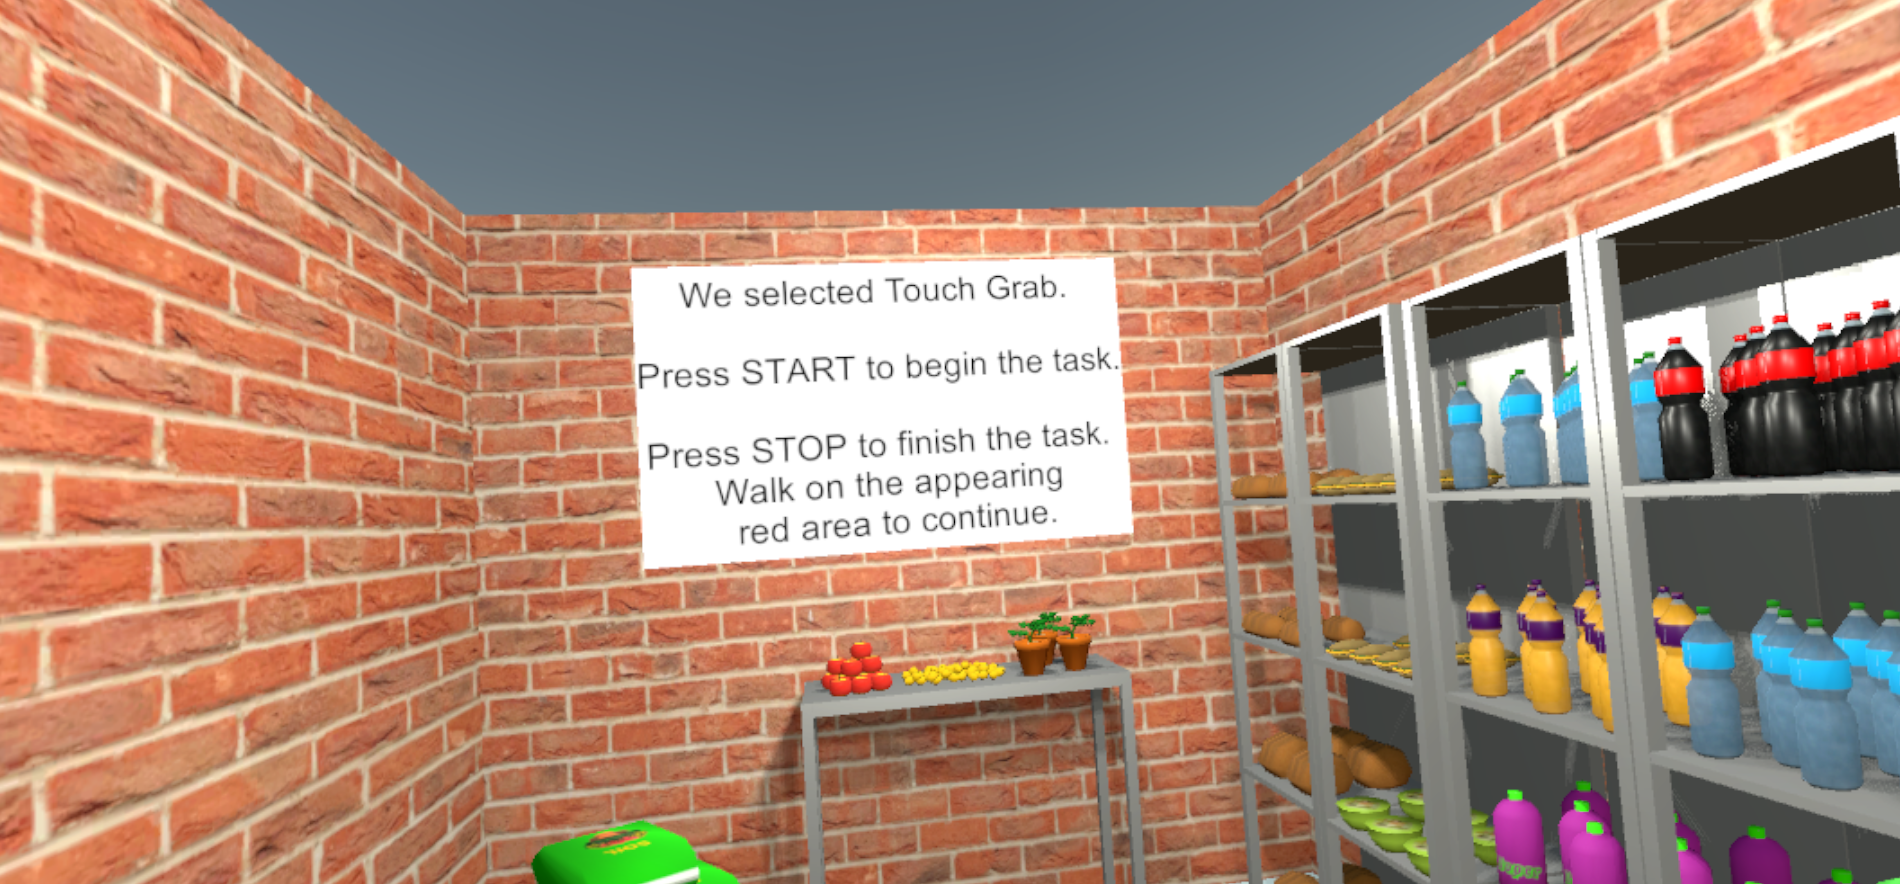
\includegraphics[width=12cm]{Images/TaskWall_2.PNG}
	\caption[Touch grab is activated]{Touch grab is activated}
	\label{fig:taskW2}
\end{figure}

In the last tasks the user has to answer an usability questionnaire about this interaction after every method. Afterwards he/she does the tasks with the next method. \\

\subsection{Measurement} \label{sec:measurement}

\subsubsection{Time and Precision Measurement}
\todo[inline, color=yellow]{Vera}
As mentioned in section \ref{sec:tasks}, several tasks had to been done by the users which are designed to evaluate various aspects. Thus, three different sets of measurements could be saved automatically in a task. All results are stored in a comma separated value text file that are named after their subtask and stored directly into the unity project folder. These files could be imported in all common statistic applications like \textit{MS Office Excel}, for example. Hence, the provided template is a \textit{Excel} file with the required basic statistic computations and visualisation of the results. Here, the output files could be easily integrated in the designated table fields. Following this, the template computes all useful mean values and standard deviations of the measurements. In other cases, it calculates the percentagewise proportion of values like the commonness of a method use. All calculations are displayed in corresponding diagrams. Further, the ones that visualise the mean values includes an error bar that depends on the standard deviation. If necessary, other static computation like a significance test needs to be extended because the calculation highly depends on the study conditions and are not predictable.

The first of the measuring sets is made for the learning room and should evaluate the affordable learning time of a grabbing method. Therefore, their usage time is stop during the complete learning process and saved in milliseconds when the user presses the stop button. 

Afterwards, the first task with its three subtasks is run. Here, the user method preference of a close or far range task should be evaluated. Hence, the application measures the usage time of every selected method and saves the id of the current method when the target object is placed successfully on the target area. The listing of this measurement shows significantly which methods were preferred and if the user had comprehensive their scope.  

Finally, the precision as well as the grabbing and positioning time is measured in the second task for every provided method. Therefore, the grabbing time is started when the user presses the start button and stopped when the user grabs the target object. At this point, the positioning time is started immediately and then stopped when the object is placed on the target area. These time measuring should show the workload and where the users have problems with the method precision. Additional, the selecting and positioning error rate is recorded during the whole process. Thus, this recorded data gives conclusions about the precision as well.  The success of this task is recorded as well as the use of the snapping mode, too. Hence, all relevant informations are provided to get all important conclusions about the applicability of each method. 


\newpage